\begin{adjustwidth*}{}{-2.25in}
\textbf{{\large Exercises}}
\setlength{\columnsep}{25pt}
\begin{multicols*}{2}
\noindent {\normalsize Problems} \small

\noindent{\bf In exercises 1--7, find the average value of the function on the given interval.}

\begin{enumerate}[1)]
\item $f(x)=\sin(x)$ on $[0,\pi/2]$
\item $y=\sin(x)$ on $[0,\pi]$
\item $y=x$ on $[0,4]$
\item $\ds f(x) = \frac{1}{1+x^2}$ on $[1,\sqrt{3}]$
\item $y=x^3$ on $[0,4]$
\item $g(t) = 1/t$ on $[1,e]$
\item $f(x) = \sec^2(x)$ on $[-\pi/4, \pi/4]$
\end{enumerate}

\noindent{\bf In exercises 8--11, find a value $c$ guaranteed by the Mean Value Theorem.}

\begin{enumerate}[1),resume]
\item $\ds \int_0^2 x^2\ dx$
\item $\ds \int_{-2}^2 x^2\ dx$
\item $\ds \int_{0}^1 e^x\ dx$
\item $\ds \int_{0}^{16} \sqrt{x}\ dx$
\end{enumerate}

\noindent{\bf In exercises 12--14, find the area of the shaded region in each given figure.}

\bmtwo
\begin{enumerate}[1),resume]
\item \noindent
\begin{minipage}{\linewidth}
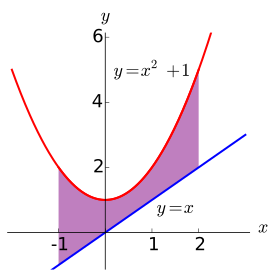
\includegraphics[scale=.35]{figs/4/4-7_Exa.pdf}
\end{minipage}

\item \noindent
\begin{minipage}{\linewidth}
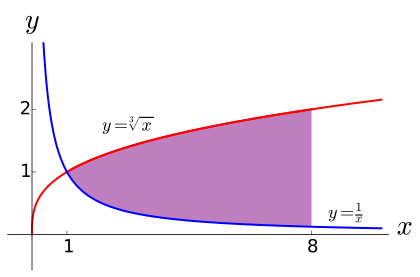
\includegraphics[scale=.35]{figs/4/4-7_Exc.pdf}
\end{minipage}

\item \noindent
\begin{minipage}{\linewidth}
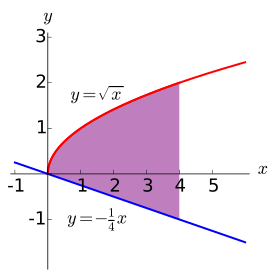
\includegraphics[scale=.35]{figs/4/4-7_Exb.pdf}
\end{minipage}
\end{enumerate}
\emtwo

\noindent{\bf In exercises 15--21, sketch the given functions and find the area of the enclosed region.}

\begin{enumerate}[1),start=15]
\item $y=2x$, $y=5x$, and $x= 3$.
\item $y=-x+1$, $y=3x+6$, $x=2$ and $x= -1$.
\item $y=x^2-2x+5$ and $y=5x-5$.
\item $y=2x^2+2x-5$ and $y=x^2+3x+7$.
\item $y = \cos(x)$ and $y = 1 - \cos(x)$ on $[0,\pi]$
\item $x = 1 - y^2$ and $x = y^2 - 1$
\item $4x + y^2 = 12$ and $x = y$

\item Suppose that the value of a car in dollars after $t$ years of use is $V(t) = 45,000e^{-0.25t}$. What is the average value of the yacht over its first $8$ years of use?

\item Water is run at a constant rate of $3$ ft$^3$/min to fill a cylindrical tank of radius $4$ ft and height $6$ ft. Assuming that the tank is initially empty, determine the average weight of the water in the tank over the time period required to fill it. Take the weight density of water to be $62.4$ lb/ft$^3$.
\end{enumerate}

%------------------------------------------
% END OF EXERCISES ON FIRST PAGE
%------------------------------------------
\end{multicols*}
\end{adjustwidth*}

%\clearpage
%
%\begin{adjustwidth*}{}{-2.25in}
%\setlength{\columnsep}{25pt}
%\begin{multicols*}{2}\small
%
%\end{enumerate}
%
%%---------------------------------------------
%% END OF EXERCISES ON SECOND PAGE
%%---------------------------------------------
%\end{multicols*}
%\end{adjustwidth*}

\afterexercises